\chapter{Diseño}
\label{cap:capitulo4}

\begin{flushright}
\begin{minipage}[]{10cm}
\emph{Quizás algún fragmento de libro inspirador...}\\
\end{minipage}\\

Autor, \textit{Título}\\
\end{flushright}

\vspace{1cm}

Escribe aquí un párrafo explicando brevemente lo que vas a contar en este capítulo. En este capítulo (y quizás alguno más) es donde, por fin, describes detalladamente qué has hecho y qué experimentos has llevado a cabo para validar tus desarrollos. Escribe aquí un párrafo explicando brevemente lo que vas a contar en este capítulo. En este capítulo (y quizás alguno más) es donde, por fin, describes detalladamente qué has hecho y qué experimentos has llevado a cabo para validar tus desarrollos.Escribe aquí un párrafo explicando brevemente lo que vas a contar en este capítulo. En este capítulo (y quizás alguno más) es donde, por fin, describes detalladamente qué has hecho y qué experimentos has llevado a cabo para validar tus desarrollos.

\section{Conectividad de los dispositivos}
\label{sec:conectividad_dispositivos}

Para realizar la conexión de todos los dispositivos entre si, se ha utilizado el switch Ethernet industrial \textbf{SCALANCE XB005\footnote{SCALANCE XB-000 unmanaged. (2025).\url{https://mall.industry.siemens.com/mall/es/es/Catalog/Product/6GK5005-0BA00-1AB2}}} y el protocolo PROFINET, el cual ya se ha explicado en la sección \ref{sec:terceraseccion}. Este dispositivo cuenta con 5 puertos, soporta cinexiones PROFINET y está pensado para usarse en fábricas o instalaciones automatizadas donde se requiere una red estable y confiable. El switch es ideal para el proyecto ya que se necesita comunicar 4 dispositivos más el ordenador que los programa entre ellos, ocupando los 5 puertos disponibles. Los cables Ethernet utilizados en son el modelo 6XV18703QN10 \footnote{6XV18703QN10. (n.d.). Radwell.eu. Retrieved June 10, 2025, from \url{https://www.radwell.eu/es/buy/siemens-6xv18703qn10/1018547.html}} los cuales son muy buenos para este tipo de aplicaciones industriales.  \\

A continuación, se muestra un diagrama de conexiones de todos los dispositivos:

\begin{figure} [h!]
  \begin{center}
    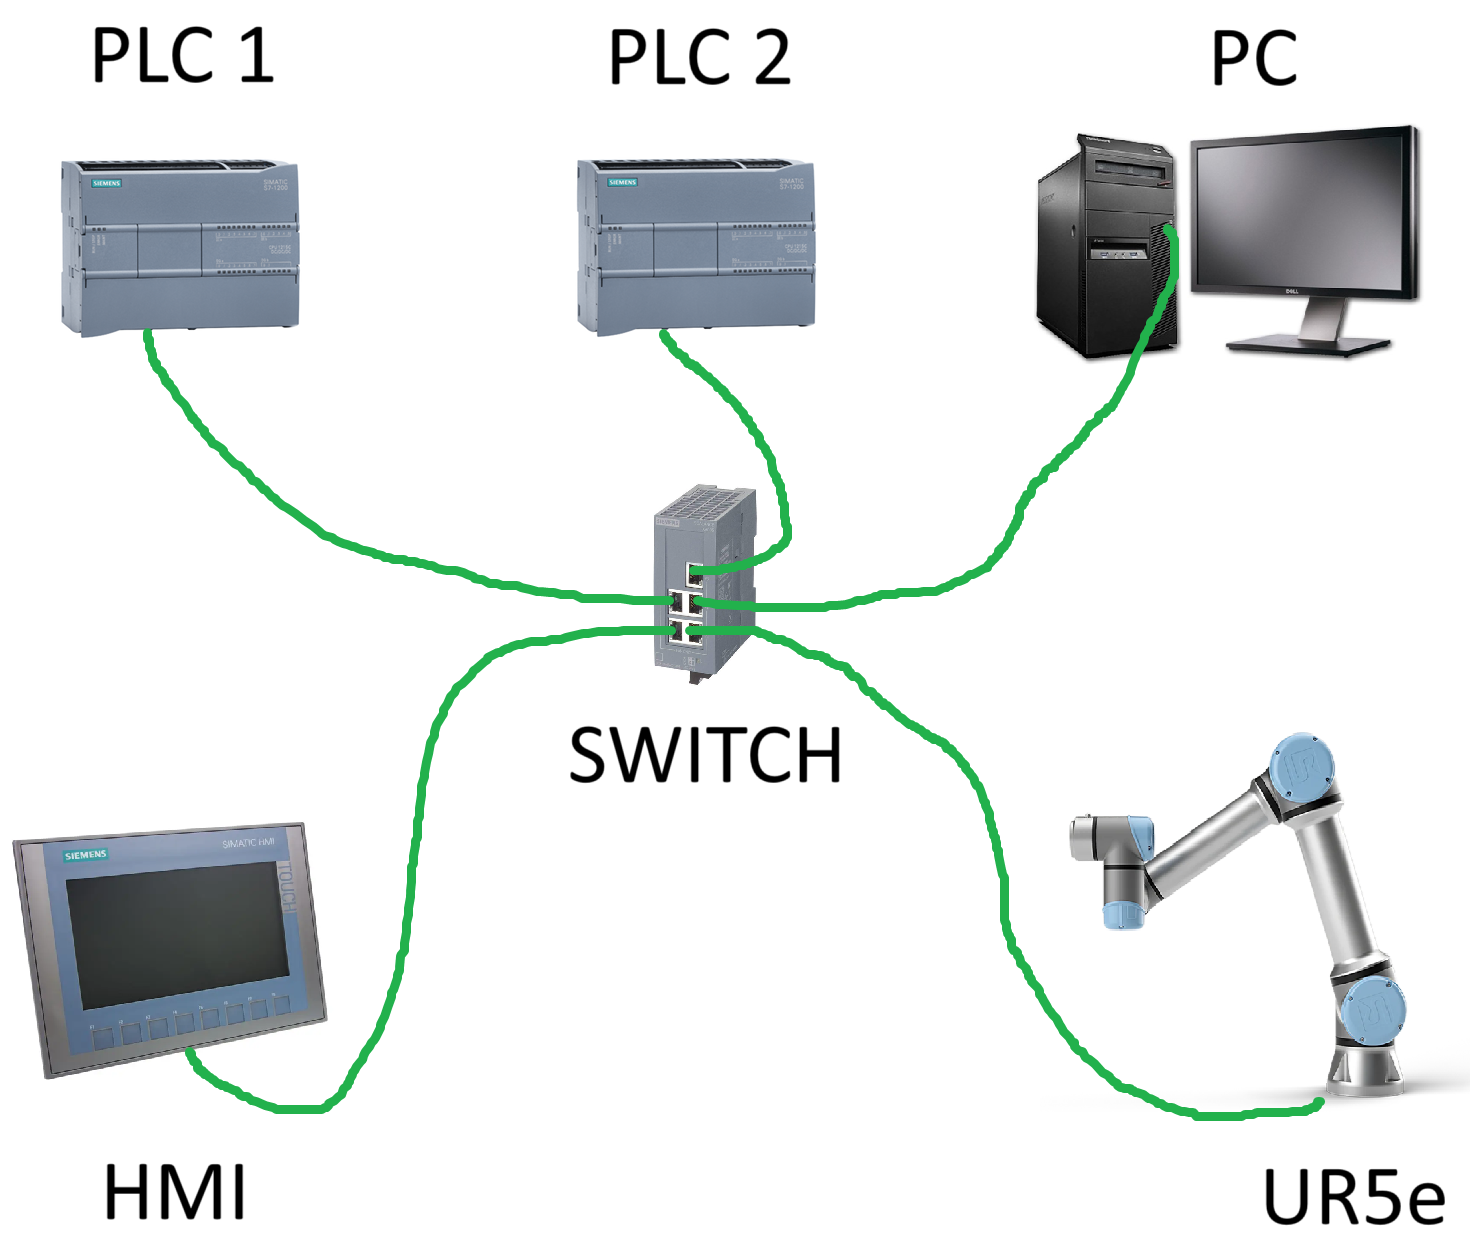
\includegraphics[width=15cm]{figs/conexion_dispositivos}
  \end{center}
  \caption{\centering Representación de conexiones entre los dispositivos del proyecto.}
  \label{fig:conexion_dispositivos}
\end{figure} 

Para intercambiar mensajes y datos entre los dos PLCs se han utilizado las funciones de comunicación RECV y SEND. SEND permite enviar información desde un PLC a otro, mientras que RECV se encarga de recibir esos datos en el destino. Estas funciones son muy útiles para coordinar procesos distribuidos y compartir datos en tiempo real en redes como Ethernet/IP o Profinet. Para la comunicación entre los PLCs, se ha definido una estructura de datos específica para cada uno, la cual se utiliza en el intercambio de mensajes. Estas estructuras contienen toda la información necesaria para el proceso, permitiendo compartir y sincronizar los datos de forma eficiente entre los distintos controladores. Cada PLC envía y recibe mensajes a una frecuencia de 5Hz y van activando o desactivando los campos de la estructura según en la etapa que se encuentren. Seguidamente se muestra una imagen de las estructuras de datos y las funciones de comunicación de los PLCs:

\clearpage

\begin{figure} [h!]
  \begin{center}
    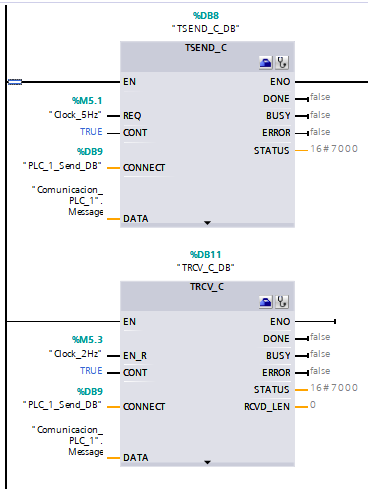
\includegraphics[width=8cm]{figs/comunicacion_plcs}
  \end{center}
  \caption{\centering Funciones SEND y RECV entre los PLCs (foto temporal).}
  \label{fig:comunicacion_plcs}
\end{figure} 

falta hablar de la comunicacion plc y ur

\section{Funcionamiento estación distribución}
\label{sec:funcionamiento_distribucion}

La estación distribución es la encargada de iniciar la secuencia del proceso automático. Esta está conectada al primer PLC y tiene como objetivo distribuir piezas al sistema, ya sea por su cinta transportadora o por el dispensador de piezas, y permitir el paso a un número determinado y tipo de piezas elegido por el usuario en el HMI. Si la pieza no cumple con las condiciones impuestas establecidas en la interfaz de usuario, esta se desplazará de vuelta al inicio descartándose, y si las cumple, continuará hacia delante a la estación distribución. También se cuenta con un modo test programado para probar el funcionamiento de cada sensor y actuador permitiendo así poder detectar errores fácilmente. A continuación se muestra una tabla en la que se reflejan todas las entradas y salidas de la estación y su conexión al PLC:

\begin{table}[H]
\begin{center}

% Tabla 1 (Sensores)
\begin{tabular}{|P{6.5cm}|P{4cm}|P{2.5cm}|}
\hline
\multicolumn{1}{|c|}{\textbf{Sensor}} & 
\multicolumn{1}{c|}{\textbf{Entrada al PLC}} & 
\multicolumn{1}{c|}{\textbf{Tipo de salida}} \\
\hline
Láser inicio cinta  & \%I0.0 &  PNP \\
Láser medio cinta  & \%I0.1 &  PNP \\
Láser final cinta  & \%I0.2 &  NPN \\
Identificador de piezas (pieza negra)  & \%I0.4 &  PNP \\
Sensor de color (pieza rosa)  & \%I0.5 &  PNP \\
Sensor metálico (pieza metálica)  & \%I0.6 &  PNP \\
Corredera retraída  & \%I0.7 &  PNP \\
Corredera extendida & \%I1.0 &  PNP \\
Pieza en el cargador & \%I1.1 &  NPN \\
\hline
\end{tabular}

\vspace{0.2cm}

% Tabla 2 (Actuadores)
\begin{tabular}{|P{6.95cm}|P{6.95cm}|}
\hline
\multicolumn{1}{|c|}{\textbf{Actuador}} & 
\multicolumn{1}{c|}{\textbf{Salida del PLC}} \\
\hline
Avance cinta & \%Q0.0 \\
Retroceso cinta & \%Q0.1 \\
Separador & \%Q0.2 \\
Avance corredera & \%Q0.3 \\
\hline
\end{tabular}

\caption{Entradas y salidas de la estación distribución conectadas al PLC 1}
\label{cuadro:distribucion}
\end{center}
\end{table}

El Grafcet de la figura \ref{fig:grafcet_distribucion} describe la secuencia automatizada de funcionamiento de la estación de unión. El sistema se inicializa con la variable de conteo de piezas a cero y permanece en espera hasta recibir una orden de arranque desde la interfaz HMI. En función del modo de carga seleccionado (manual o automático), se activa el avance de la cinta transportadora mediante un separador temporizado o a través de la corredera que realiza un movimiento de extensión y retracción para depositar la pieza retenida en el cargador. A continuación, se lleva a cabo una etapa de identificación en la que se determina el tipo de pieza (negra, rosa o metálica), registrándose dicha información en el sistema y actualizándose el contador de piezas correspondiente. El HMI cuenta con una interfaz para seleccionar el tipo de pieza que se quiere aceptar y la que se quiere descartar, como se observa en la imagen \ref{fig:HMI_funcionamiento}, en la que con esa configuración los tres tipos de piezas serían descartados. Si se ha alcanzado el número total de piezas especificado por el operador o el tipo de pieza no está permitida por el operario, el sistema ejecuta un retroceso de la cinta para descartar la pieza y repetir el ciclo hasta que se reseté el contador de piezas o se amplíe el número desde el HMI. En caso contrario, se da por finalizado el proceso de carga, se envía una señal al PLC 2 informando de la finalización de la secuencia y el tipo de pieza detectada, se espera su respuesta para asegurar que ha recibido el mensaje y termina el ciclo. 

\clearpage

\begin{figure} [h!]
  \begin{center}
    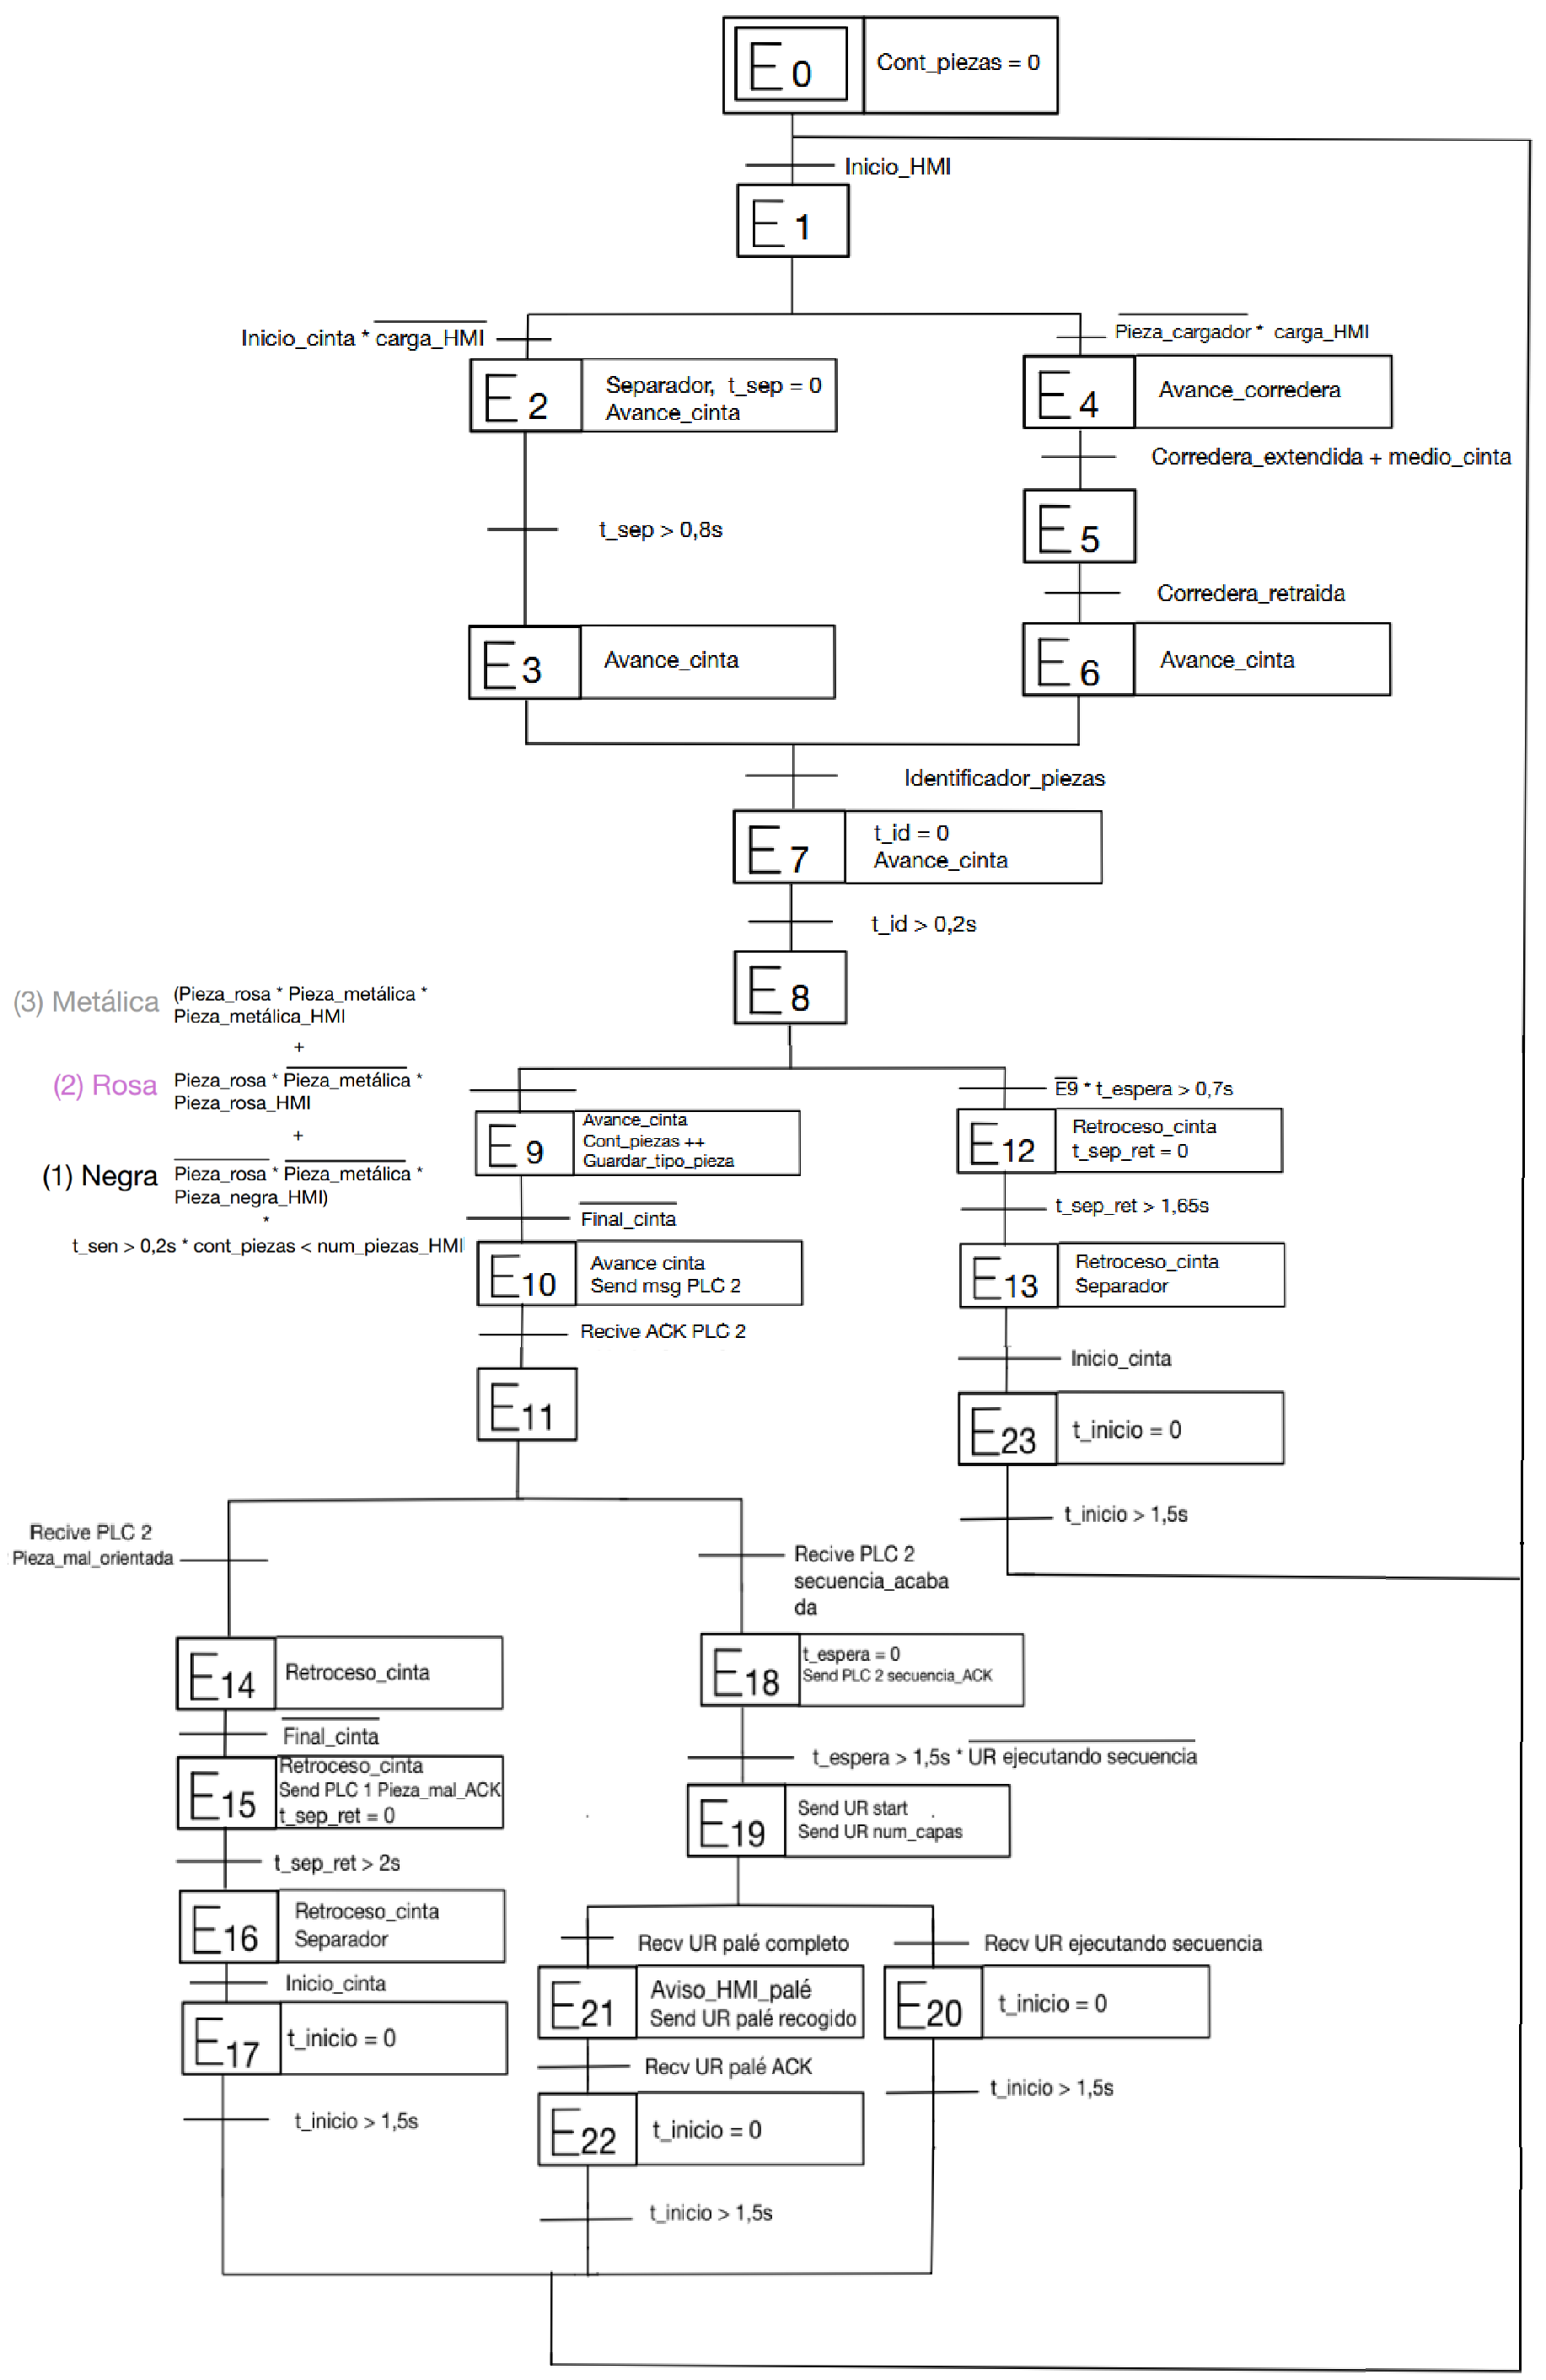
\includegraphics[width=15cm]{figs/grafcet_distribucion}
  \end{center}
  \caption{\centering Grafcet del funcionamiento de la estación distribución.}
  \label{fig:grafcet_distribucion}
\end{figure} 

\clearpage

\begin{figure} [h!]
  \begin{center}
    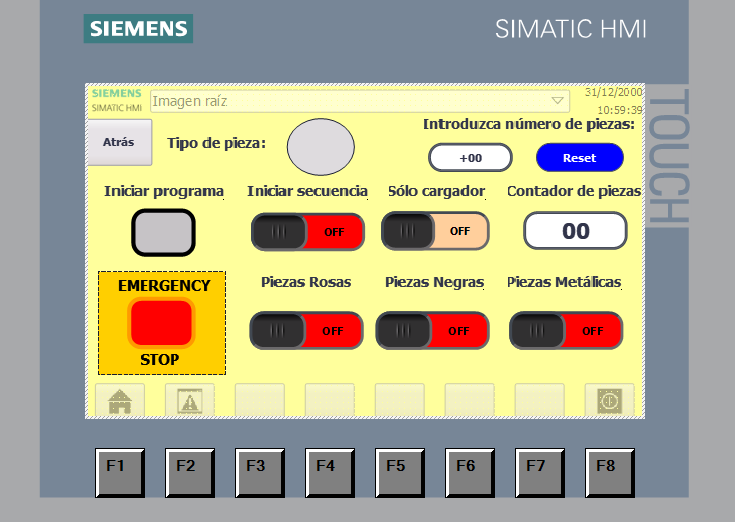
\includegraphics[width=15cm]{figs/HMI_funcionamiento}
  \end{center}
  \caption{\centering Modo funcionamiento en el HMI.}
  \label{fig:HMI_funcionamiento}
\end{figure} 

\section{Funcionamiento estación unión}
\label{sec:funcionamiento_union}

La estación unión es la encargada de ensamblar las diferentes piezas que llegan desde las estaciones anteriores, formando así subconjuntos dentro del proceso automatizado. Esta estación se encuentra conectada al segundo PLC del sistema y tiene como objetivo principal unir una base con una tapa, verificando previamente que ambas piezas estén correctamente posicionadas. El proceso de unión se realiza mediante un actuador neumático equipado con una ventosa, este puede desplazarse entre las dos cintas para así ascender y descender para recoger o dejar las tapas. En caso de que alguna de las piezas esté mal posicionada, el sistema detendrá el ciclo, notificará el error mediante un mensaje en la pantalla del HMI y posteriormente descartará la pieza. Esta estación también cuenta con un modo test que permite revisar individualmente el funcionamiento de cada sensor y actuador, facilitando la identificación de posibles fallos mecánicos o de programación. A continuación, se muestra la tabla \ref{cuadro:union} en la que se detallan todas las entradas y salidas de la estación y su conexión al PLC:

\begin{table}[H]
\begin{center}

% Tabla 1 (Sensores)
\begin{tabular}{|P{6.5cm}|P{4cm}|P{2.5cm}|}
\hline
\multicolumn{1}{|c|}{\textbf{Sensor}} & 
\multicolumn{1}{c|}{\textbf{Entrada al PLC}} & 
\multicolumn{1}{c|}{\textbf{Tipo de salida}} \\
\hline
Láser inicio cinta 1 & \%I0.0 &  PNP \\
Láser medio cinta 1  & \%I0.1 &  PNP \\
Láser final cinta 1  & \%I0.2 &  NPN \\
Orientación correcta  & \%I0.3 &  PNP \\
Láser final cinta 2 & \%I0.4 &  PNP \\
Láser inicio cinta 2 & \%I0.5 &  NPN \\
Carro retraido & \%I0.6 &  PNP \\
Carro extendido & \%I0.7 &  PNP \\
Ventosa arriba & \%I1.0 &  PNP \\
Pieza succionada & \%I1.1 &  PNP \\

\hline
\end{tabular}

\vspace{0.2cm}

% Tabla 2 (Actuadores)
\begin{tabular}{|P{6.95cm}|P{6.95cm}|}
\hline
\multicolumn{1}{|c|}{\textbf{Actuador}} & 
\multicolumn{1}{c|}{\textbf{Salida del PLC}} \\
\hline
Avance cinta 1 & \%Q0.0 \\
Retroceso cinta  2 & \%Q0.1 \\
Extender derivador & \%Q0.2 \\
Retraer tope & \%Q0.3 \\
Avance cinta 2 & \%Q0.4 \\
Retroceso cinta 2 & \%Q0.5 \\
Retroceso carro & \%Q0.6 \\
Avance carro & \%Q0.7 \\
Bajar ventosa & \%Q1.0 \\
Vacío conectado & \%Q1.1 \\
\hline
\end{tabular}

\caption{Entradas y salidas de la estación unión conectadas al PLC 2}
\label{cuadro:union}
\end{center}
\end{table}

El grafcet de la estación distribución puede observarse en la figura \ref{fig:grafcet_union}, cuya función es colocarle una tapa a las provenientes de la estación de distribución encima de ellas, siempre y cuando estén bien orientadas.  El proceso comienza activando el avance de la cinta 1 hasta que la pieza proveniente de la estación distribución es detectada por el láser del inicio, después, se envía un mensaje al PLC 1 de respuesta de confirmación de que la pieza ha llegado al segundo sistema. La cinta continúa moviéndose hasta que es detectada en el centro de la cinta por el segúndo láser y se extiende el retenedor para poder así comprobar correctamente la orientación de la pieza. A continuación se verifica la orientación de la pieza utilizando un sensor capacitivo que responde de forma inversa a las piezas metálicas: si la pieza está correctamente orientada, el sensor no la detecta, mientras que si está invertida, el sensor la activa, indicando una orientación incorrecta. Si se confirma que la orientación es válida, paralelamente se dan dos sucesos: en el primero se vuelve a activar la cinta 1, se extiende el derivador y se espera el tiempo necesario para que la pieza llegue hasta este último y el segundo consiste en que la cinta 2 avanza hasta que en el láser del inicio de esta detecta una tapa. Una vez está la pieza parada y la tapa lista para ser recogida, el carro se extiende, desciende la ventosa, succiona la pieza, se eleva y se retrae colocándola encima de la pieza. Después la ventosa se desactiva, se activa la cinta 1 nuevamente y se retrae el derivador permitiendo a la pieza llegar al final de la cinta, que, cuando es detectada por el último láser le manda un mensaje al PLC 1 indicándole que la secuencia ha terminado. Si la orientación es incorrecta, se activa un proceso de rechazo y se activa una notificación al operario mediante el HMI informando que la pieza es defectuosa y mostrando un contador de ellas. El sistema se quedará esperando hasta que el operario le de al botón de ``descartar pieza'' como se observa en la imagen  \ref{fig:HMI_descarte}, una vez pulsado el botón, se activa el retroceso de la cinta 1 y el envío de un mensaje de error al PLC 1 avisándole de que debe descartar la pieza. El ciclo finaliza tras la confirmación de recepción de la secuencia completada o de pieza defectuosa por parte del PLC 1. \\

\begin{figure}[h!]
  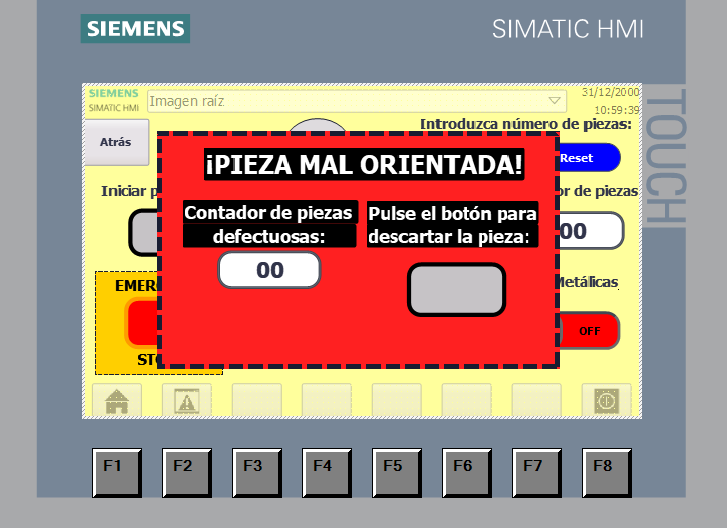
\includegraphics[width=16cm]{figs/HMI_descarte}
  \caption{\centering Aviso de pieza defectuosa en el modo funcionamiento en el HMI.}
  \label{fig:HMI_descarte}
\end{figure}

\begin{figure}[h!]
  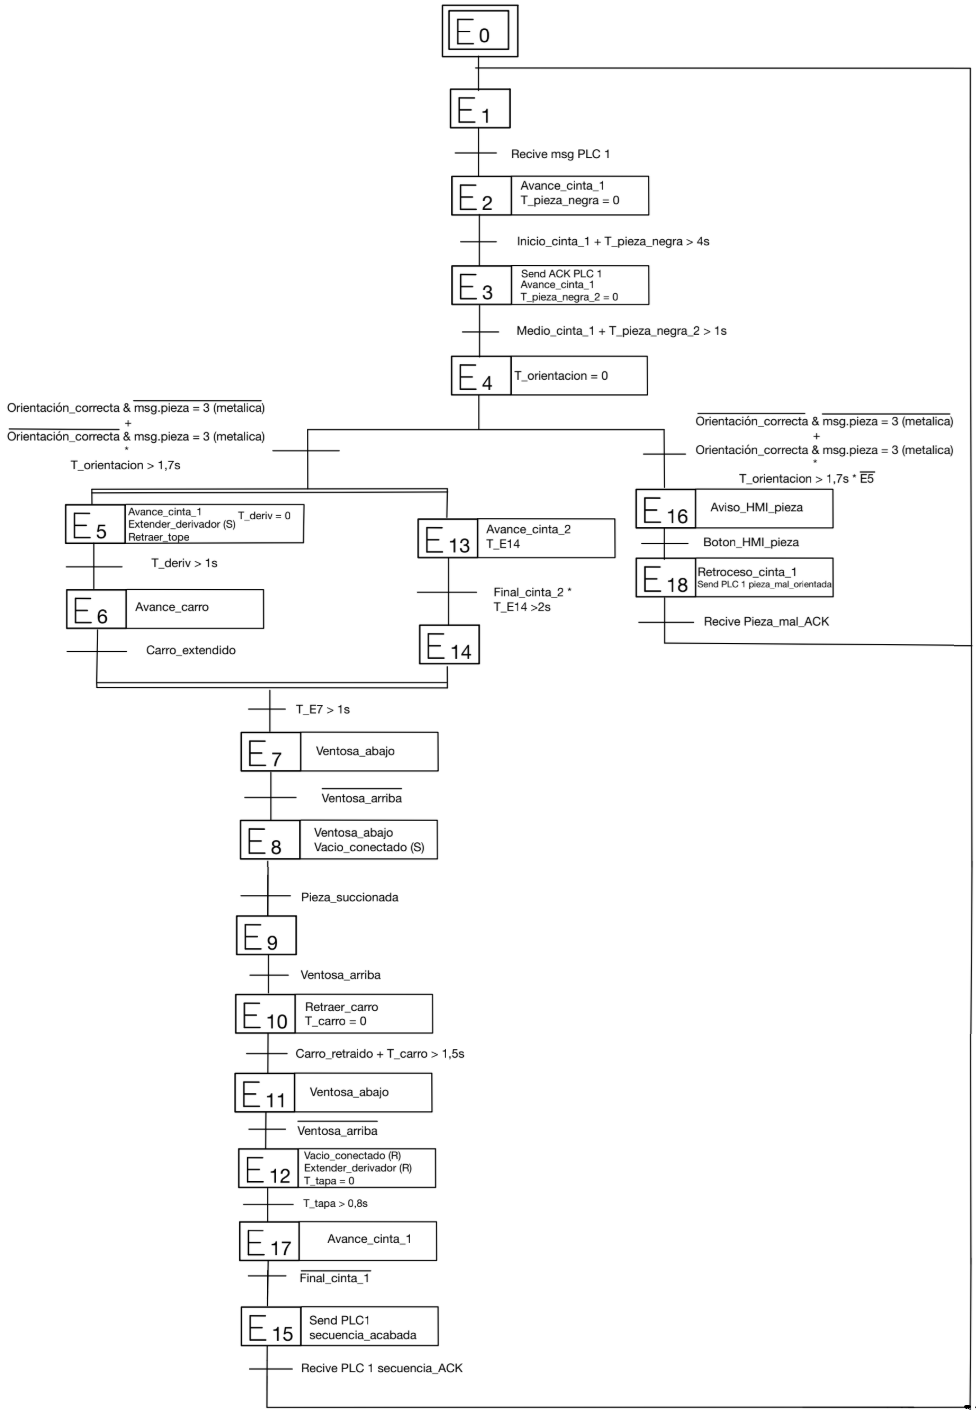
\includegraphics[width=15cm]{figs/grafcet_union}
  \caption{\centering Grafcet de funcionamiento de la estación unión.}
  \label{fig:grafcet_union}
\end{figure}

\clearpage


\section{Aplicación de la Guía Gemma}
\label{sec:aplicacion_gemma}

La aplicación de la Guía Gemma explicada en la sección \ref{sec:terceraseccion} es un aspecto muy importante a la hora de programar las estaciones si se quiere obtener un resultado funcional, seguro y estructurado.  Facilita la identificación de modos de funcionamiento, fallos y transiciones entre estados. Para la aplicación de la Guía Gemma en el proyecto se han utilizado los siguientes estados:

\begin{table}[H] 
\begin{center}

\renewcommand{\arraystretch}{1.5}
\begin{tabular}{|P{3.5cm}|P{4cm}|P{7cm}|}
\hline
\textbf{Modo} & \textbf{Tipo} & \textbf{Objetivo} \\
\hline

\multirow{2}{=}{Proceso de funcionamiento} 
    & F1: Producción normal & Se realizan las tareas principales del sistema. \\
\cline{2-3}
    & F4: Marchas de verificación sin orden & Se realiza un control manual de los actuadores y la comprobación del funcionamiento de los sensores. \\
\hline

\multirow{3}{=}{Proceso de parada o puesta en marcha} 
    & A1: Parada en el estado inicial & Estado de reposo de la máquina. \\
\cline{2-3}
    & A2: Parada solicitada al final de ciclo & Estado al que se llega  cuando se termina el ciclo y pasa al estado inicial\\
\cline{2-3}
    & A3: Parada solicitada en un estado determinado & Estado al que llega la máquina alternativo el cual no coincide con el final de ciclo. \\
\cline{2-3}
    & A4: Parada obtenida & Estado de reposo diferente al principal. \\
\hline

Proceso en defecto & D1: Parada de emergencia & Estado al que llega el sistema tras una parada de emergencia. Se para el funcionamiento de todo el sistema. \\
\hline

\end{tabular}

\caption{Estados de la Guía Gemma utilizados en el sistema.}
\label{cuadro:union}
\end{center}
\end{table}

\subsubsection{Proceso de funcionamiento}


\subsubsection{Proceso de parada o puesta en marcha}


\subsubsection{Proceso en defecto}

\clearpage

\section{Funcionamiento cobot UR5e}
\label{sec:funcionamiento_ur5e}

El cobot UR5e es un brazo robótico colaborativo diseñado para trabajar de forma segura junto a operarios. En este proyecto, su función principal es comunicarse con los PLCs para ejecutar una secuencia de paletizado en la fase final del ciclo global del sistema. Una vez que la estación de distribución completa su ciclo, el PLC 1 envía una señal al UR5e indicándole que inicie su secuencia. Al finalizar la operación de paletizado, el cobot notifica al PLC 1 que ha concluido, permitiendo así reiniciar el ciclo completo. El propósito de integrar el brazo en la ejecución del sistema es simular su uso dentro del proceso automático (aunque físicamente no se pudo integrar debido a la distancia entre estaciones) y aportar así mayor realismo y complejidad al resultado final. 

El cobot viene equipado con una pinza neumática como herramienta. Esta pinza permite sujetar, mover y soltar objetos de forma rápida y eficiente. Es ideal para tareas repetitivas como ensamblaje, paletizado, manipulación de piezas o carga de máquinas, especialmente cuando no se requiere un control preciso de la fuerza. Esta pinza se ha utilizado para la secuencia de paletizado, la cual siguie el esquema llamado \textbf{paletizado por capas}. Este tipo de paletizado por capas consiste en organizar productos sobre un palé formando niveles horizontales uniformes agrupando varios elementos alineados o alternos para lograr estabilidad \cite{paletizado_capas}. Es ideal para cargas regulares y facilita la automatización, optimizando espacio, transporte y manipulación en entornos industriales \cite{paletizado_capas}. 

\begin{figure}[h!]
  \begin{center}
  	\includegraphics[width=11.5cm]{figs/brazo_pinza}
  \end{center}
  \caption{\centering UR5e junto con la pinza como herramienta.}
  \label{fig:brazo_pinza}
\end{figure}

Como ya se ha visto en la sección \ref{sec:conectividad_dispositivos}, el PLC 1 le envía un mensaje al UR para iniciar el programa de paletizado. En este programa se ha utilizado la herramienta de paletizado integrada en Polyscope. Esta funcionalidad permite crear un palé de cualquier tipo de elemento indicando únicamente el número de capas deseadas y las coordenadas de la posición de cada uno. Tal como se ha mencionado anteriormente, se ha llevado a cabo un paletizado por capas, utilizando bricks de leche como elementos a colocar, simulando una secuencia real en un entorno industrial. Se han configurado cuatro capas en total: dos con una disposición determinada y las otras dos con una diferente, obteniendo el siguiente resultado:

\begin{figure}[h!]
  \begin{center}
  	\includegraphics[width=15cm]{figs/resultado_paletizado}
  \end{center}
  \caption{\centering Resultado final del paletizado de bricks de leche por el UR5e.}
  \label{fig:resultado_paletizado}
\end{figure}

Las coordenadas de la posición de los bricks de leche en el paletizado se han tomado de forma relativa a la coordenada del primer brick de leche. La primera coordenada se definió en la posición que se quería colocar el primer elemento del palet, y a partir de esta y tomándola de referencia, se han definido las 5 coordenadas restantes. Al utilizar el sistema de coordenadas del primer punto se han podido colocar elementos paralelos y perpendiculares al primero, ayudando ha aportar gran estabilidad y orden al palet. Esta técnica ha ayudado mucho también a establecer la misma altura de todos los bricks de leche y asegurarse así que no se coloquen de forma uniforme. Adicionalmente se han establecido algunos puntos de paso también en este sistema de coordenadas para intentar establecer los movimientos lo más rectilíneos posibles. 

\textbf{NOTA}: Qué es mejor opción de poner a continuación?: las coordenadas de los bricks de leche (por foto o tabla), una imagen del código del UR o ambas.

\clearpage
\section{Diseño del sistema SCADA}
\label{sec:diseño_scada}



\section{Resultado final}
\label{sec:resultado_final}





